\documentclass{article}
\usepackage[utf8]{inputenc}
\usepackage[spanish]{babel}
\usepackage{graphicx}
\usepackage{geometry}
\usepackage{enumerate}
\usepackage{titlesec}
\usepackage{float}
\usepackage{listings}
\usepackage{xcolor}
\usepackage{amsmath}
\usepackage{matlab-prettifier}
\usepackage{amssymb}
\usepackage{tabularx}

\geometry{letterpaper, margin = 1.5cm}

\newcommand{\codefontsize}{\fontsize{10}{11}}
\lstset{
	style = Matlab-editor,
	basicstyle = \codefontsize\ttfamily,
	mlshowsectionrules = true,
	upquote = true,
	tabsize = 4,
	captionpos = b,
	breaklines = true,
	breakatwhitespace = true,
	frame = single,
}

%Datos de la Portada
\title{Introducción a la Programación \ Practica 6}
\author{Medina Martinez Jonathan Jason \ 2023640061}
\date{22 de abril del 2023}

\begin{document}
	
	\fontsize{12}{16}\selectfont
	
	\begin{figure}[t]
		
		
\includegraphics[width=2.5 cm]{Logo1.jpeg}
		\hfill
		
\includegraphics[width=3 cm]{Logo2.png}
		
	\end{figure}
	
	\maketitle
	\newpage
	
	\tableofcontents
	\newpage
	
	\section{Objetivo}
	
	Crear los diferentes tipos de gráficos bidimensionales y tridimensionales existentes en lenguaje de programación científico.
	
	\section{Introducción}
	
	
	En la práctica número 6 de Herramientas Computacionales se trabajarán los diferentes tipos de gráficos bidimensionales y tridimensionales existentes en lenguaje de programación científico. A través de un \textbf{script}, se crearán gráficas para diferentes funciones matemáticas, ajustando sus características visuales y generando una figura con múltiples subgráficas. 
	
	\newpage
	\section{Desarrollo}
	
	Escriba un Script para cada uno de los siguientes puntos.
	
	\subsection{Problema 1}
	
	Cree graficas de las siguientes funciones, desde x = 0 hasta 10.

	\begin{equation*}
		y = e^{x}
	\end{equation*}
	
	\begin{equation*}
		y = \sin(x)
	\end{equation*}
	
	\begin{equation*}
		y = ax^2 + bx + c, \text{ donde } a = 5, b = 2 \text{ y } c = 4
	\end{equation*}
	
	\begin{equation*}
		y = \sqrt{x}
	\end{equation*}
	
	Cada una de sus graficas debe incluir titulo, etiqueta del eje x, etiqueta del eje y y un \textbf{grid}.
	
	\newpage
	
	\subsubsection{Script1.m}
	
	\begin{lstlisting}
	
	% Programa que grafica la funcion y = e^x desde x = 0 hasta x = 10.
	
	x = 0:0.1:10;
	
	y = exp(x);
	figure
	plot(x, y)
	title('Grafica de y = e^x')
	xlabel('x')
	ylabel('y')
	grid on
	\end{lstlisting}
	
	\subsubsection{Ejecución}
	
	\begin{lstlisting}
	>> Script1
	\end{lstlisting}
	
	\subsubsection{Grafica 1}
	
	\begin{figure*}[h]
	\centering
	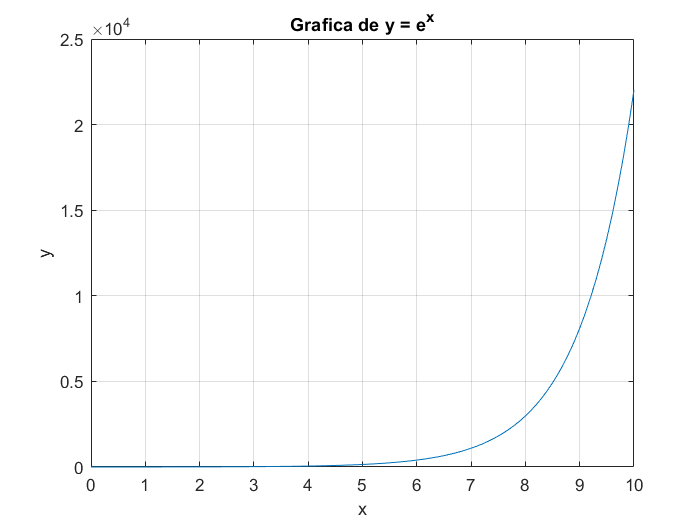
\includegraphics[width=\textwidth]{grafica1.png}
	\end{figure*}
	
	\subsubsection{Script2.m}
	
	\begin{lstlisting}
% Programa qque grafica la funcion y = sin(x) desde x = 0 hasta x = 10.

x = 0:0.1:10;

y = sin(x);
figure
plot(x, y)
title('Grafica de y = sin(x)')
xlabel('x')
ylabel('y')
grid on
	\end{lstlisting}
	
	\subsubsection{Ejecución}
	
	\begin{lstlisting}
		>> Script2
	\end{lstlisting}
	
	\subsubsection{Grafica 2}
	
	\begin{figure*}[h]
		\centering
		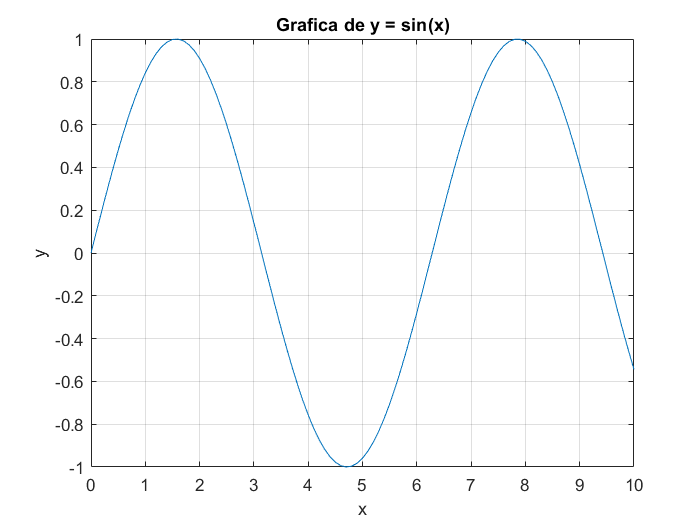
\includegraphics[width=\textwidth]{grafica2.png}
	\end{figure*}
	
	\newpage
	
	\subsubsection{Script3.m}
	
	\begin{lstlisting}
% Programa que grafica la funcion y = 5x^2 + 2x + 4  desde x=0 hasta x=10.

x = 0:0.1:10;

a = 5;
b = 2;
c = 4;
y = a*x.^2 + b*x + c;
figure
plot(x, y)
title('Grafica de y = 5x^2 + 2x + 4')
xlabel('x')
ylabel('y')
grid on
	\end{lstlisting}
	
	\subsubsection{Ejecución}
	
	\begin{lstlisting}
		>> Script3
	\end{lstlisting}
	
	\subsubsection{Grafica 3}
	
	\begin{figure*}[h]
		\centering
		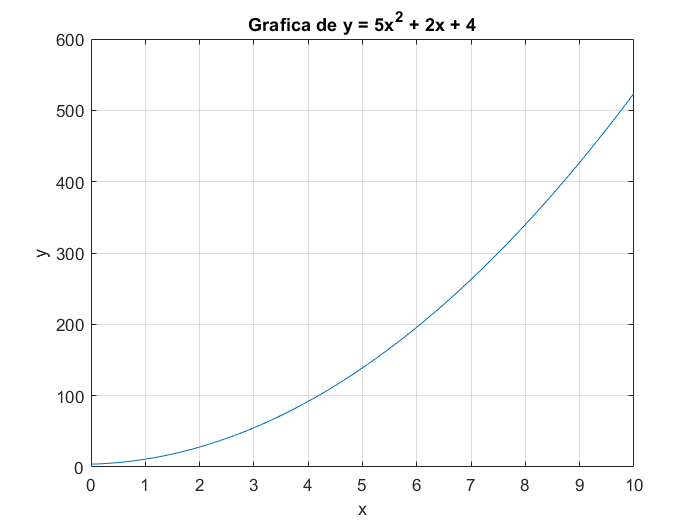
\includegraphics[width=\textwidth]{grafica3.png}
	\end{figure*}
	
	\newpage
	
	\subsubsection{Script4.m}
	
	\begin{lstlisting}
% Programa que grafica la y = nthroot(x,2) desde x = 0 hasta x = 10.

x = 0:0.1:10;

y = nthroot(x,2);
figure
plot(x, y)
title('Grafica de y = nthroot(x,2)')
xlabel('x')
ylabel('y')
grid on
	\end{lstlisting}
	
	\subsubsection{Ejecución}
	
	\begin{lstlisting}
		>> Script4
	\end{lstlisting}
	
	\subsubsection{Grafica 4}
	
	\begin{figure*}[h]
		\centering
		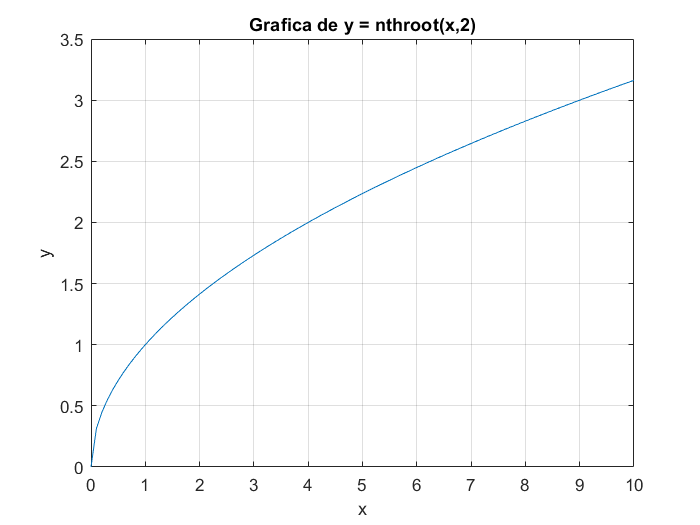
\includegraphics[width=\textwidth]{grafica4.png}
	\end{figure*}
	
	\subsection{Problema 2}
	
	
	Representa la función $f(x) =  \frac{1.5*x}{x-4}$ para $-10 <= x <= 10$. Observe que esta función posee una asíntota vertical en el punto $x = 4$. Represente la función mediante la creacion de dos vectores para el dominio de $x$. El primer vector ($x1$) contendrá los elementos $-10$ a $3.7$, y el segundo vector ($x2$) los elementos $4.3$ hasta $10$.
	
	Adicionalmente habrá que crear dos vectores $y1$ e $y2$ para las correspondencias con los valores de la función sobre los dos vectores anteriormente creados para el dominio de $x$.
	
	Seguidamente represente la función mediante dos curvas en la misma grafica.
	
	\subsubsection{Script5.m}
	
	\begin{lstlisting}
		
% Programa que genera la grafica de la funcion f(x) = 1.5x / (x - 4) desde
% x = -10 a 10.

x1 = -10:0.1:3.7;
x2 = 4.3:0.1:10;

y1 = 1.5*x1./(x1-4);
y2 = 1.5*x2./(x2-4);

plot(x1,y1,'b',x2,y2,'b','LineWidth',2)

xlabel('x','FontSize',14)
ylabel('y','FontSize',14)

title('Grafica de la funcion f(x)= 1.5x / (x - 4)','FontSize',16)

grid on

xlim([-10,10])
ylim([-18.5,20])

hold on

plot([0,0],[-20,20],'k-','LineWidth',0.5)

plot([-10,10],[0,0],'k-','LineWidth',0.5)

hold off

legend('f(x)','Location','NorthWest')

	\end{lstlisting}
	
	\subsubsection{Ejecución}
	
	\begin{lstlisting}
		>> Script5
	\end{lstlisting}
	
	\newpage
	
	\subsubsection{Grafica}
	
	\begin{figure*}[h]
		\centering
		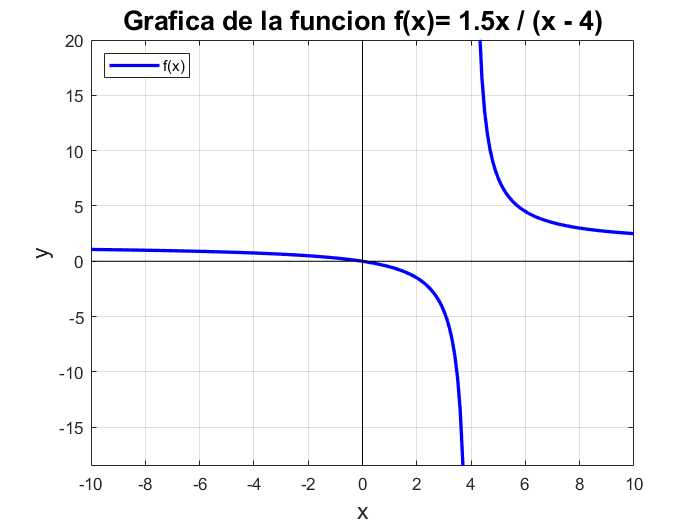
\includegraphics[width=\textwidth]{grafica5.png}
	\end{figure*}
	
	\newpage
	
	\subsection{Problema 3}
	
	Grafique las siguientes funciones en la misma grafica para valores de $x$ desde $-\pi$ hasta $\pi$, y seleccione el espaciamiento para crear una grafica suave:
	
	\begin{itemize}
		\centering
		\item $y1 = \sin(x)$
		\item $y2 = \sin(2x)$
		\item $y3 = \sin(3x)$
	\end{itemize}
	
	\subsubsection{Script6.m}
	
	\begin{lstlisting}

% Programa que genera una grafica las siguientes funciones:
% -> f(x) = sin(x)
% -> f(x) = sin(2x)
% -> f(x) = sin(3x)
% Todas dentro de una misma grafica.

x = -pi:0.00001: pi;
y1 = sin(x);
y2 = sin(2.*x);
y3 = sin(3.*x);

hold on

plot(x, y1, 'LineWidth', 1.5)
plot(x, y2, 'LineWidth', 1.5)
plot(x, y3, 'LineWidth', 1.5)

hold off

xlabel('x')
ylabel('y')

grid on

xlim([-pi, pi])
ylim([-1, 1])

title('Grafica de la funciones sin(x), sin(2x), sin(3x)')
legend('sin(x)', 'sin(2x)', 'sin(3x)','Location','NorthWest')

	\end{lstlisting}	
	
	\subsubsection{Ejecución}
	
	\begin{lstlisting}
		>> Script6
	\end{lstlisting}
	
	\newpage
	
	\subsubsection{Grafica}
	
	\begin{figure*}[h]
		\centering
		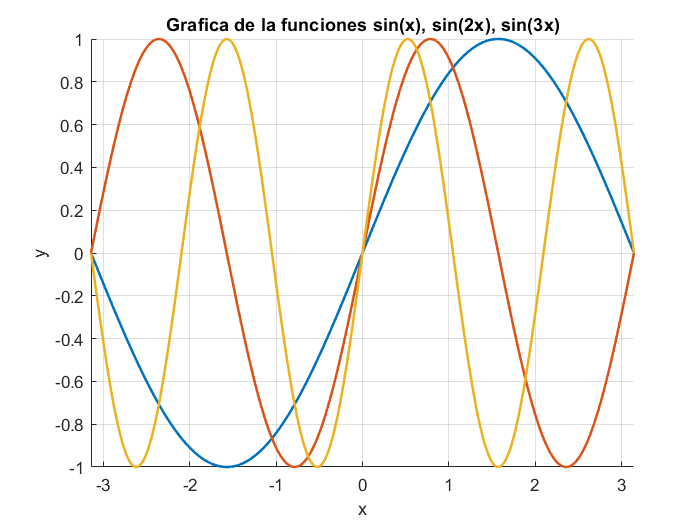
\includegraphics[width=\textwidth]{grafica6.png}
	\end{figure*}
	
	\newpage
	
	\subsection{Problema 4}
	
	Ajuste la grafica creada en el problema anterior de modo que
	\begin{itemize}
		\item La linea 1 sea roja y rayada.
		\item La linea 2 sea azul y solida.
		\item La linea 3 sea verde y punteada.
	\end{itemize}
	No incluya marcadores en ninguna de las graficas.
	\subsubsection{Script7.m}
	
	\begin{lstlisting}

% Programa que genera una grafica las siguientes funciones:
%
% -> f(x) = sin(x)
% -> f(x) = sin(2x)
% -> f(x) = sin(3x)
% 
% Todas dentro de una misma grafica, con el siguiente formato:
%
% -> La linea 1 es roja y rayada.
% -> La linea 2 es azul y solida.
% -> La linea 3 es verde y punteada.

x = (-1*pi): 0.00001: (pi);

y1 = sin(x);
y2 = sin(2.*x);
y3 = sin(3.*x);

hold on

plot(x, y1, 'r--', 'LineWidth', 3)
plot(x, y2, 'b-', 'LineWidth', 3)
plot(x, y3, 'g:', 'LineWidth', 3)

hold off

xlabel('x')
ylabel('y')

grid on

xlim([(-1*pi), pi])
ylim([-1, 1])

title('Grafica de la funciones sin(x), sin(2x), sin(3x)')

	\end{lstlisting}
	
	\subsubsection{Ejecución}
	
	\begin{lstlisting}
		>> Script7
	\end{lstlisting}
	
	\newpage
	
	\subsubsection{Grafica}
	
	\begin{figure*}[h]
		\centering
		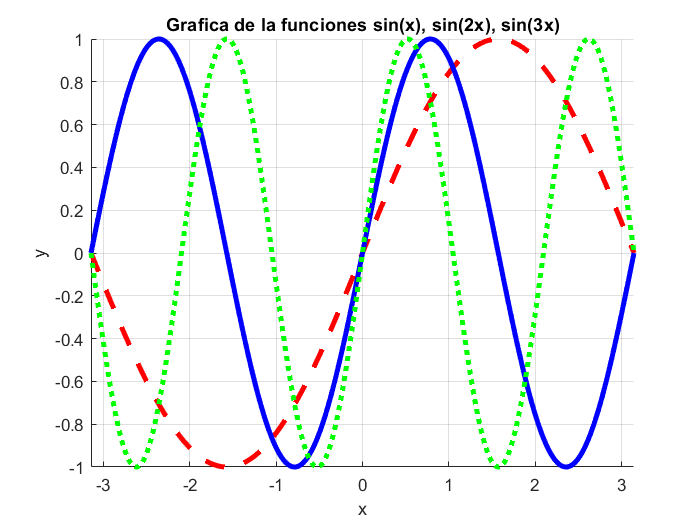
\includegraphics[width=\textwidth]{grafica7.png}
	\end{figure*}
	
	\newpage
	
	\subsection{Problema 5}
	
	Ajuste la grafica creada en el problema anterior de modo que el eje $x$ vaya desde $-4$ hasta $4$. Agregue una leyenda y un recuadro de texto que describa las graficas.
	
	\subsubsection{Script8.m}
	
	\begin{lstlisting}

% Programa que genera una grafica las siguientes funciones:
%
% -> f(x) = sin(x)
% -> f(x) = sin(2x)
% -> f(x) = sin(3x)
% 
% Todas dentro de una misma grafica, con el siguiente formato:
%
% -> La linea 1 es roja y rayada.
% -> La linea 2 es azul y solida.
% -> La linea 3 es verde y punteada.

x = (-4): 0.00001: (4);

y1 = sin(x);
y2 = sin(2.*x);
y3 = sin(3.*x);

hold on

plot(x, y1, 'r--', 'LineWidth', 1.5)
plot(x, y2, 'b-', 'LineWidth', 1.5)
plot(x, y3, 'g:', 'LineWidth', 1.5)

hold off

xlabel('x')
ylabel('y')

grid on

xlim([-4, 4])
ylim([-1, 1])

title('Grafica de las funciones sin(x), sin(2x), sin(3x)')

legend({'sin(x)', 'sin(2x)', 'sin(3x)'}, 'Location', 'southwest')

dim = [.57 .75 .25 .15];
str = {'Linea 1: roja y rayada', 'Linea 2: azul y solida', 'Linea 3: verde y punteada'};
annotation('textbox', dim, 'String', str, 'FitBoxToText', 'on');

	\end{lstlisting}
	
	\subsubsection{Ejecución}
	
	\begin{lstlisting}
		>> Script8
	\end{lstlisting}
	
	\newpage
	
	\subsubsection{Grafica}
	
	\begin{figure*}[h]
		\centering
		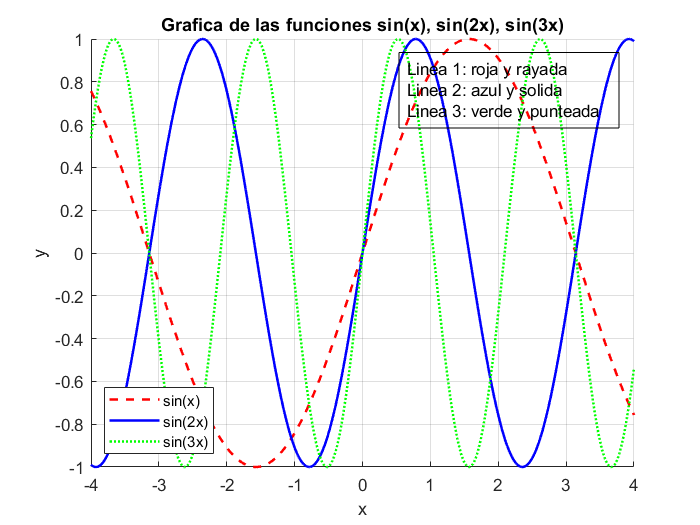
\includegraphics[width=\textwidth]{grafica8.png}
	\end{figure*}
	
	\newpage
	
	\subsection{Problema 6}
	
	En el problema 1, creo cuatro graficas. Combınelas en una figura con cuatro subgraficas, con la función \textbf{subplot} de MATLAB.
	
	\subsubsection{Script9.m}
	
	\begin{lstlisting}

% Programa que genera subgraficas dentro de una misma grafica.

x = 0:0.1:10;

y1 = exp(x);

y2 = sin(x);

a = 5; b = 2; c = 4;
y3 = a*x.^2 + b*x + c;

y4 = sqrt(x);


figure
subplot(2,2,1)
plot(x, y1, 'b-', 'LineWidth', 2)
title('Funcion exponencial')
xlabel('x')
ylabel('y')
grid on

subplot(2,2,2)
plot(x, y2, 'r-', 'LineWidth', 2)
title('Funcion seno')
xlabel('x')
ylabel('y')
grid on

subplot(2,2,3)
plot(x, y3, 'g-', 'LineWidth', 2)
title('Funcion cuadratica')
xlabel('x')
ylabel('y')
grid on

subplot(2,2,4)
plot(x, y4, 'm-', 'LineWidth', 2)
title('Funcion raiz cuadrada')
xlabel('x')
ylabel('y')
grid on

	\end{lstlisting}
	
	\subsubsection{Ejecución}
	
	\begin{lstlisting}
		>> Script9
	\end{lstlisting}
	
	\newpage
	
	\subsubsection{Grafica}
	
	\begin{figure*}[h]
		\centering
		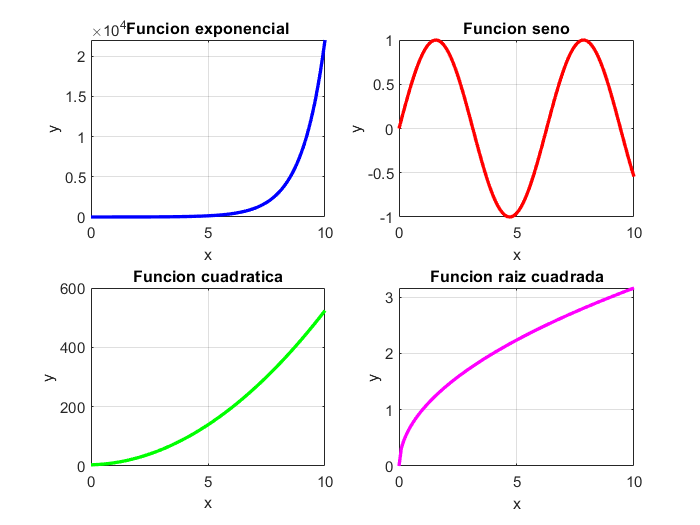
\includegraphics[width=\textwidth]{grafica9.png}
	\end{figure*}
	
	\newpage
	
	\subsection{Problema 7}
	
	Represente la función $f(x) = 3x \sin(x)-2x$ y su derivada, ambas en la misma grafica, en el intervalo $-2\pi \leq x \leq 2\pi$. Represente la función con una linea solida, y su derivada con una linea discontinua. Añada una leyenda y etiquetas para los ejes.
	
	\subsubsection{Script10.m}
	
	\begin{lstlisting}
		
% Programa que grafica la funcion f(x) = 3*x*sin(x) - 2*x y su derivada.

x = -2*pi:0.00001:2*pi;

f = 3*x.*sin(x) - 2*x;

df = 3*sin(x) + 3*x.*cos(x) - 2;

figure

hold on

plot(x, f, 'LineWidth', 2)
plot(x, df, '--', 'LineWidth', 2)

hold off

legend('Funcion', 'Derivada')

xlabel('x')
ylabel('y')

grid on

	\end{lstlisting}
	
	\subsubsection{Ejecución}
	
	\begin{lstlisting}
		>> Script10
	\end{lstlisting}
	
	\newpage
	
	\subsubsection{Grafica}
	
	\begin{figure*}[h]
		\centering
		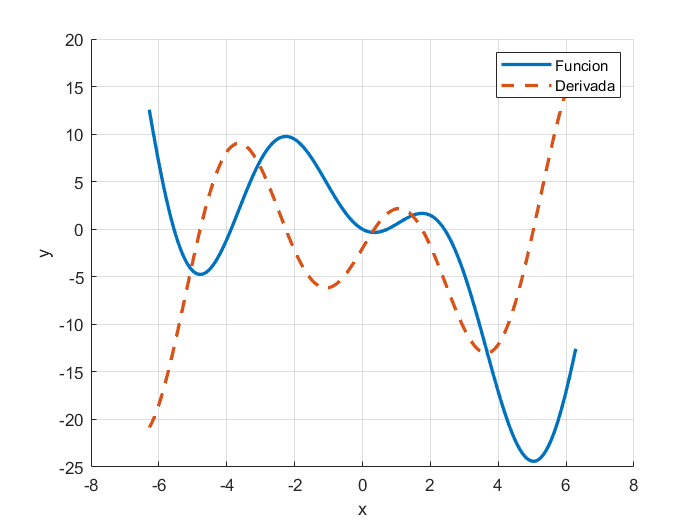
\includegraphics[width=\textwidth]{grafica10.png}
	\end{figure*}
	
	\newpage
	
	\subsection{Problema 8}
	
	Tome las ecuaciones del ejercicio 3 y grafíquelas en una sola figura con cuatro subgraficas y graficas polares.
	
	\subsubsection{Script11.m}
	
	\begin{lstlisting}

% Programa que geneara las graficas polares de las funciones del Script6.m

theta = 0:0.01:2*pi;
yp1 = sin(theta);
yp2 = sin(2*theta);
yp3 = sin(3*theta);

figure;
subplot(2,2,1)
polarplot(theta, yp1, 'r-', 'LineWidth', 2)
title('sin(\theta)')

subplot(2,2,2)
polarplot(theta, yp2, 'b-', 'LineWidth', 2)
title('sin(2\theta)')

subplot(2,2,3)
polarplot(theta, yp3, 'g-', 'LineWidth', 2)
title('sin(3\theta)')

subplot(2,2,4)
polarplot(theta, yp1, 'r-', 'LineWidth', 1)
hold on
polarplot(theta, yp2, 'b-', 'LineWidth', 1)
polarplot(theta, yp3, 'g-', 'LineWidth', 1)
title('Todas en una')
hold off

	\end{lstlisting}
	
	\subsubsection{Ejecución}
	
	\begin{lstlisting}
		>> Script11
	\end{lstlisting}
	
	\newpage
	
	\subsubsection{Grafica}
	
	\begin{figure*}[h]
		\centering
		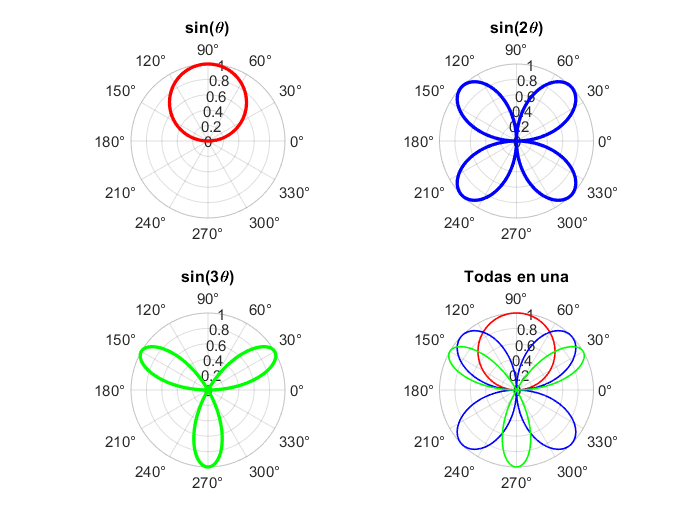
\includegraphics[width=\textwidth]{grafica11.png}
	\end{figure*}
	
	\newpage
	
	\subsection{Problema 9}
	
	Basándose en el ejercicio anterior:
	
	\begin{enumerate}[a)]
		\item Cree una “flor” con tres pétalos.
		\\
		\item Superponga su figura con ocho pétalos adicionales de la mitad del tamaño de los tres originales.
		\\
		\item Cree un corazón.
		\\
		\item Cree una estrella de seis puntas.
		\\
		\item Cree un hexágono.
		\\
	\end{enumerate}
		
	\newpage
	
	\subsubsection{Script12.m}
	
	\begin{lstlisting}

% Programa que genera una flor de 3 petalos.

theta = 0:(0.01):(2*pi);
y = sin(3*theta);

polarplot(theta, y, 'm-', 'LineWidth', 10)

ax = gca;
ax.ThetaAxis.Visible = 'off';
ax.RAxis.Visible = 'off';

	\end{lstlisting}

	\subsubsection{Ejecución}
	
	\begin{lstlisting}
		>> Script12
	\end{lstlisting}
	
	\subsubsection{Grafica}
	
	\begin{figure*}[h]
		\centering
		
\includegraphics[width=\textwidth]{grafica12.png}
	\end{figure*}
	
	\newpage
	
	\subsubsection{Script13.m}
	
	\begin{lstlisting}
% Programa que genera una flor de 3 petalos y otra flor de 8 petalos.

theta = 0:(0.01):(2*pi);
y1 = sin(3*theta);
y2 = 0.5*sin(4*theta);

polarplot(theta, y1, 'm-', 'LineWidth', 5)

hold on
polarplot(theta, y2, 'b-', 'LineWidth', 5)
hold off

ax = gca;
ax.ThetaAxis.Visible = 'off';
ax.RAxis.Visible = 'off';
	\end{lstlisting}
	
	\subsubsection{Ejecución}
	
	\begin{lstlisting}
		>> Script13
	\end{lstlisting}
	
	\subsubsection{Grafica}
	
	\begin{figure*}[h]
		\centering
		
\includegraphics[width=\textwidth]{grafica13.png}
	\end{figure*}
	
	\subsubsection{Script14.m}
	
	\begin{lstlisting}

% Programa que grafica un corazon.

t = 0:(0.01):(2*pi);

x = 12*sin(t).^3;
y = 13*cos(t) - 5*cos(2*t) - 2*cos(3*t) - cos(4*t);

fill(x, y, 'r');

axis off;

	\end{lstlisting}
	
	\subsubsection{Ejecución}
	
	\begin{lstlisting}
		>> Script14
	\end{lstlisting}
	
	\subsubsection{Grafica}
	
	\begin{figure*}[h]
		\centering
		
\includegraphics[width=\textwidth]{grafica14.png}
	\end{figure*}

	\newpage
	
	\subsubsection{Script15.m}
	
	\begin{lstlisting}

% Programa grafica una estrella.

x = linspace(-2*pi,2*pi,1000);
X = pi/2:4/5*pi:4.8*pi;
Y = ones(1,6);

polarplot(X,Y,'c','LineWidth',2)

rlim([0 1.2])

title('Grafica de la estrella')
	\end{lstlisting}
	
	\subsubsection{Ejecución}
	
	\begin{lstlisting}
		>> Script15
	\end{lstlisting}
	
	\subsubsection{Grafica}
	
	\begin{figure*}[h]
		\centering
		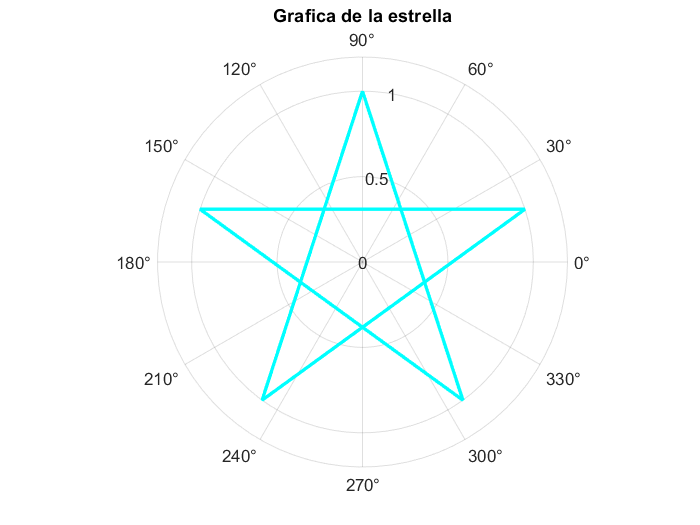
\includegraphics[width=\textwidth]{grafica15.png}
	\end{figure*}
	
	\newpage
	
	\subsubsection{Script16.m}
	
	\begin{lstlisting}
% Programa que genera la grafica de un Hexagono.

theta = linspace(0, 2*pi, 7);

x = cos(theta);
y = sin(theta);

plot(x, y, 'b', 'LineWidth', 2)
axis equal
	\end{lstlisting}
	
	\subsubsection{Ejecución}
	
	\begin{lstlisting}
		>> Script16
	\end{lstlisting}
	
	\subsubsection{Grafica}
	
	\begin{figure*}[h]
		\centering
		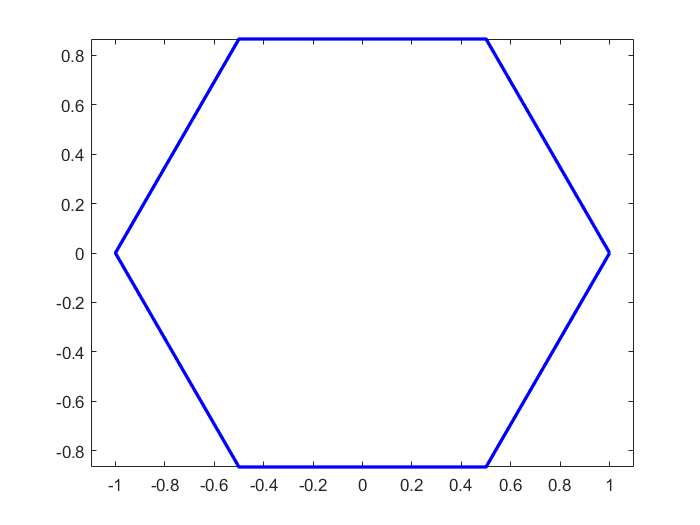
\includegraphics[width=\textwidth]{grafica16.png}
	\end{figure*}
	
	\newpage
	
	\subsection{Problema 10}
	
	La orbita de los planetas alrededor del Sol se puede modelar, de forma aproximada, mediante la siguiente ecuación polar:
	
	\begin{equation*}
		r(\theta) = \frac{\alpha(1-\sqrt{e})}{1-e\cos(\theta)}
	\end{equation*}
	
	Donde:
	
	\begin{itemize}
		\item $r$ es la distancia.
		\item $\alpha$ es el semieje mayor, que define el tamaño de la orbita.
		\item $e$ es la excentricidad orbital, que define la forma de la orbita.
		\item $\theta$ es el angulo entre la posición actual del objeto en orbita y la ubicación en la orbita en la que esta mas cerca del cuerpo central.
	\end{itemize}
	
	\subsubsection{Script17.m}
	
	\begin{lstlisting}

% Programa que grafica las orbitas de los planetas del sistema solar.

theta = 0:(0.01):(2*pi);

polarplot(theta, orbita(0.3871, 0.206), 'w--', 'LineWidth', 1, 'DisplayName', 'Mercurio')
hold on

polarplot(theta, orbita(0.7233, 0.007), 'c--', 'LineWidth', 1, 'DisplayName', 'Venus')
polarplot(theta, orbita(1.000, 0.017), 'y--', 'LineWidth', 1, 'DisplayName', 'Tierra')
polarplot(theta, orbita(1.5273, 0.093), 'm--', 'LineWidth', 1, 'DisplayName', 'Marte')
polarplot(theta, orbita(5.2028, 0.048), 'g--', 'LineWidth', 1, 'DisplayName', 'Jupiter')
polarplot(theta, orbita(9.5388, 0.056), 'b--', 'LineWidth', 1, 'DisplayName', 'Saturno')
polarplot(theta, orbita(19.1914, 0.046), 'r--', 'LineWidth', 1, 'DisplayName', 'Urano')
polarplot(theta, orbita(30.0611, 0.010), 'k--', 'LineWidth', 1, 'DisplayName', 'Neptuno')

hold off

legend('show')

set(gca, 'Color', [0.2 0.3 0.7])

ax = gca;

ax.ThetaAxis.Visible = 'off';

ax.RAxis.Visible = 'off';

grid off

	\end{lstlisting}
	
	\subsubsection{orbita.m}
	
	\begin{lstlisting}
function res = orbita(a, e)

theta = 0:(0.01):(2*pi);

res = (a*(1-(e*e)))./(1+(e*cos(theta)));
	\end{lstlisting}

	\subsubsection{Ejecución}
	
	\begin{lstlisting}
	>>Script17
	\end{lstlisting}
	
	\subsubsection{Grafica}
	
	\begin{figure*}[h]
		\centering
		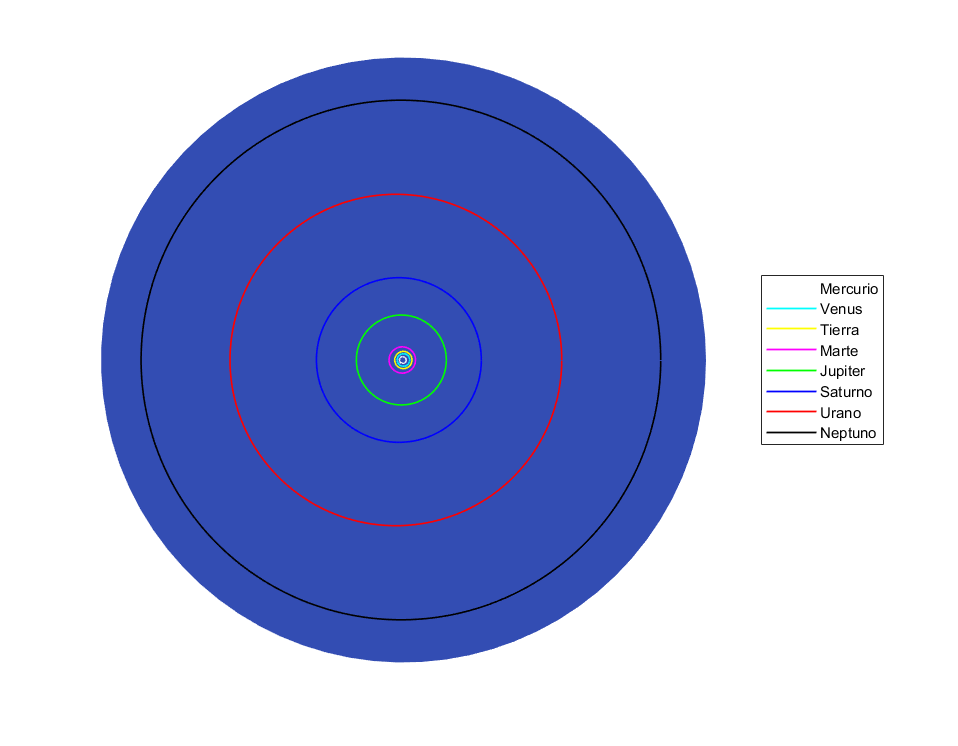
\includegraphics[width=\textwidth]{grafica17.png}
	\end{figure*}
	
	\newpage
	
	\subsection{Problema 11}
	
	De acuerdo con la ley de Moore (una observación hecha en 1965 por Gordon Moore, cofundador de Intel Corporation), el numero de transistores que encajaría por pulgada cuadrada en un circuito integrado semiconductor se duplica aproximadamente cada 18 meses. El año 2022 fue el 57 aniversario de la ley. Durante los últimos 57 años, su proyección se ha satisfecho de manera consistente. En 1965, la entonces tecnología de avanzada permitía 30 transistores por pulgada cuadrada. La ley de Moore dice que la densidad de transistores se puede predecir mediante $d(t) = 30(2\frac{t}{1.5})$, donde $t$ se mide en años.
	
	\begin{itemize}
		\item Sea $t = 0$ la representación del año 1965 y $t = 57$ la representación de 2022. Use este modelo para calcular el numero predicho de transistores por pulgada cuadrada para los 57 años desde 1965 hasta 2022. Sea $t$ el aumento en incrementos de 1.5 años. Muestre los resultados en una tabla con 2 columnas, una para el año y otra para el numero de transistores.
		\item Con el comando subplot, grafique los datos en una grafica lineal $x - y$, una grafica x semilog, una grafica y semilog y una grafica $log-log$. Asegúrese de poner titulo y etiqueta a los ejes.
	\end{itemize}
	
	\subsubsection{Script18.m}
	
	\begin{lstlisting}

% Programa que genera una tabla con la estimacion del numero de
% transistores para anios proximos cada medio anio y , a su vez, genera
% graficas del crecimiento en cantidad que estos tendrian.

d = @(t) 30 * 2^(t/1.5);

datos = zeros(38, 2);

for i = 1:38
t = (i-1)*1.5; 
anio = 1965 + t;
transistores = d(t);
datos(i,:) = [anio, transistores];
end

tabla = array2table(datos, 'VariableNames', {'Anio', 'Numero de transistores'});
disp(tabla);

figure;

subplot(2,2,1);
plot(datos(:,1), datos(:,2), 'r-', 'LineWidth', 2.5);
title("Grafico lineal");

subplot(2,2,2);
semilogx(datos(:,1), datos(:,2), 'b-', 'LineWidth', 2.5);
title("Grafico x semilog");

subplot(2,2,3);
semilogy(datos(:,1), datos(:,2), 'c-', 'LineWidth', 2.5);
title("Grafico y semilog");

subplot(2,2,4);
loglog(datos(:,1), datos(:,2), 'm-', 'LineWidth', 2.5);
title("Grafico log-log");


	\end{lstlisting}
	
	\newpage
	
	\subsubsection{Ejecución}
	
	\begin{lstlisting}
	
	>>Script18
	Anio     Numero de transistores
	______    ______________________
	
	1965                  	30    
	1966.5                  60      
	1968               	   120      
	1969.5             	   240      
	1971               	   480      
	1972.5                 960      
	1974                  1920      
	1975.5                3840      
	1977                  7680      
	1978.5               15360      
	1980                 30720      
	1981.5               61440      
	1983            1.2288e+05      
	1984.5          2.4576e+05      
	1986            4.9152e+05      
	1987.5          9.8304e+05      
	1989            1.9661e+06      
	1990.5          3.9322e+06      
	1992            7.8643e+06      
	1993.5          1.5729e+07      
	1995            3.1457e+07      
	1996.5          6.2915e+07      
	1998            1.2583e+08      
	1999.5          2.5166e+08      
	2001            5.0332e+08      
	2002.5          1.0066e+09      
	2004            2.0133e+09      
	2005.5          4.0265e+09      
	2007            8.0531e+09      
	2008.5          1.6106e+10      
	2010            3.2212e+10      
	2011.5          6.4425e+10      
	2013            1.2885e+11      
	2014.5           2.577e+11      
	2016             5.154e+11      
	2017.5          1.0308e+12      
	2019            2.0616e+12      
	2020.5          4.1232e+12      
	
	\end{lstlisting}
	
	\newpage
	
	\subsubsection{Grafica}
	
	\begin{figure*}[h]
		\centering
		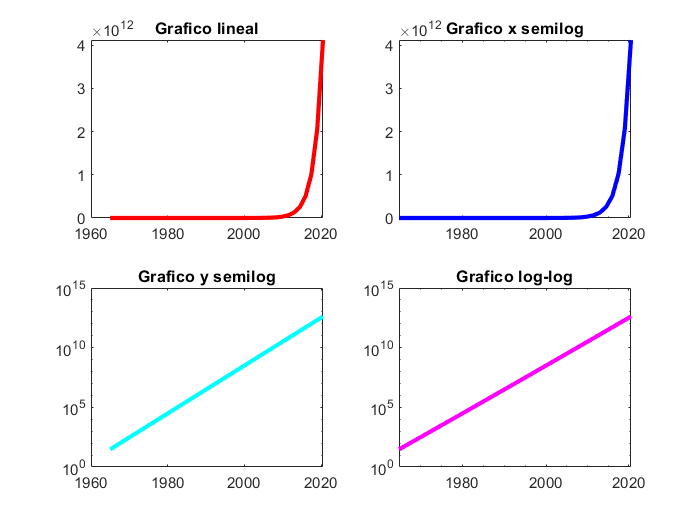
\includegraphics[width=\textwidth]{grafica18.png}
	\end{figure*}
	
	\newpage
	
	\subsection{Problema 12}
	
	Sea el vector $G = [6.8, 8.3, 6.1, 7.0, 7.5, 8.2, 5.7, 5.0, 7.6, 8.5, 6.2, 7.1, 9.6, 7.8, 7.6, 6.8, 7.2, 7.5, 8.3, 9.3]$ que representa la distribución de calificaciones finales en un curso de Herramientas Computacionales.
	
	\begin{enumerate}
		\item Use MATLAB para ordenar los datos y cree una grafica de barras de las calificaciones.
		\item Cree un histograma de las calificaciones.
	\end{enumerate}
	
	\subsubsection{Script19.m}
	
	\begin{lstlisting}

% Programa que usando el vector G de unas calificaciones dadads las ordena
% y grafica.

G = [6.8, 8.3, 6.1, 7.0, 7.5, 8.2, 5.7, 5.0, ...
7.6, 8.5, 6.2, 7.1, 9.6, 7.8, 7.6, 6.8, 7.2, 7.5, 8.3, 9.3];

ord = sort(G);

figure;
bar(ord);
xlabel('Estudiantes');
ylabel('Calificaciones');
title('Distribucion de Calificaciones');

figure;
histogram(G, 'Normalization', 'count');
xlabel('Calificaciones');
ylabel('Frecuencia Relativa');
title('Histograma de Calificaciones');

	\end{lstlisting}
	
	\subsubsection{Ejecución}
	
	\begin{lstlisting}
	>>Script19
	\end{lstlisting}
	
	\newpage
	
	\subsubsection{Grafica 1}
	
	\begin{figure*}[h]
		\centering
		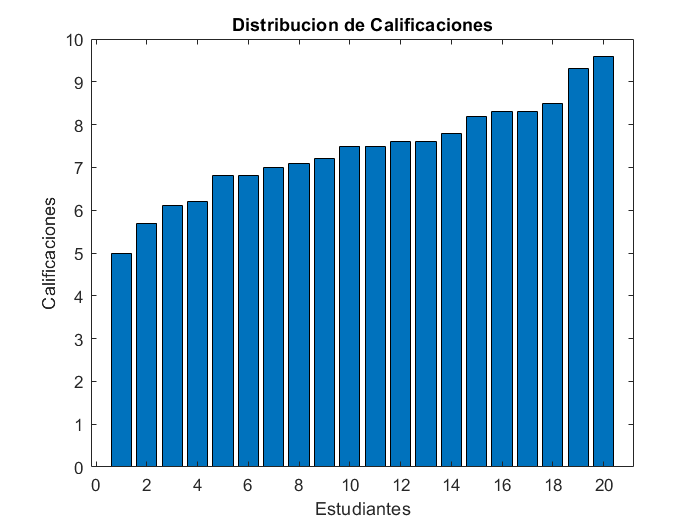
\includegraphics[width=\textwidth]{grafica19a.png}
	\end{figure*}
	
	\newpage
	
	\subsubsection{Grafica 2}
	
	\begin{figure*}[h]
		\centering
		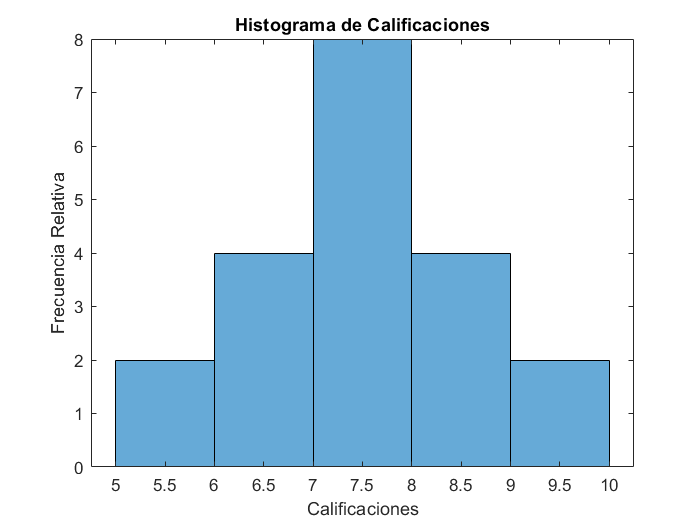
\includegraphics[width=\textwidth]{grafica19b.png}
	\end{figure*}
	
	\newpage
	
	\subsection{Problema 13}
	
	En la clase de Herramientas Computacionales del ejercicio anterior, pudo notar que hay:
	\begin{itemize}
		\item 2 calificaciones grado A (9 - 10)
		\item 4 calificaciones grado B (8 - 9)
		\item 8 calificaciones grado C (7 - 8)
		\item 4 calificaciones grado D (6 - 7)
		\item 2 calificaciones grado E (5 - 6)
	\end{itemize}
	
	\begin{enumerate}[a)]
		\item Cree una grafica de pastel de esta distribución. Agregue una leyenda que mencione los nombres de calificación (A, B, C, D, E).
		\item Cree una grafica de pastel tridimensional de los mismos datos.
	\end{enumerate}
	
	\subsubsection{Script20.m}
	
	\begin{lstlisting}

% Programa que genera dos graficas de pastel 2d y 3d con el numero de 
% estudiantes que obtuvierion ciertas calificaciones en el ejercicio
% anterior.

n = [2, 4, 8, 4, 2];

figure;
pie(n);
legend('A', 'B', 'C', 'D', 'E');
title('Distribucion de Calificaciones en Herramientas Computacionales');

% Grafica de pastel tridimensional
figure;
pie3(n);
legend('A', 'B', 'C', 'D', 'E');
title('Distribucion de Calificaciones en Herramientas Computacionales (3D)');

	\end{lstlisting}
	
	\subsubsection{Ejecución}
	
	\begin{lstlisting}
	>>Script23
	\end{lstlisting}
	
	\newpage
	
	\subsubsection{Grafica 1}
	
	\begin{figure*}[h]
		\centering
		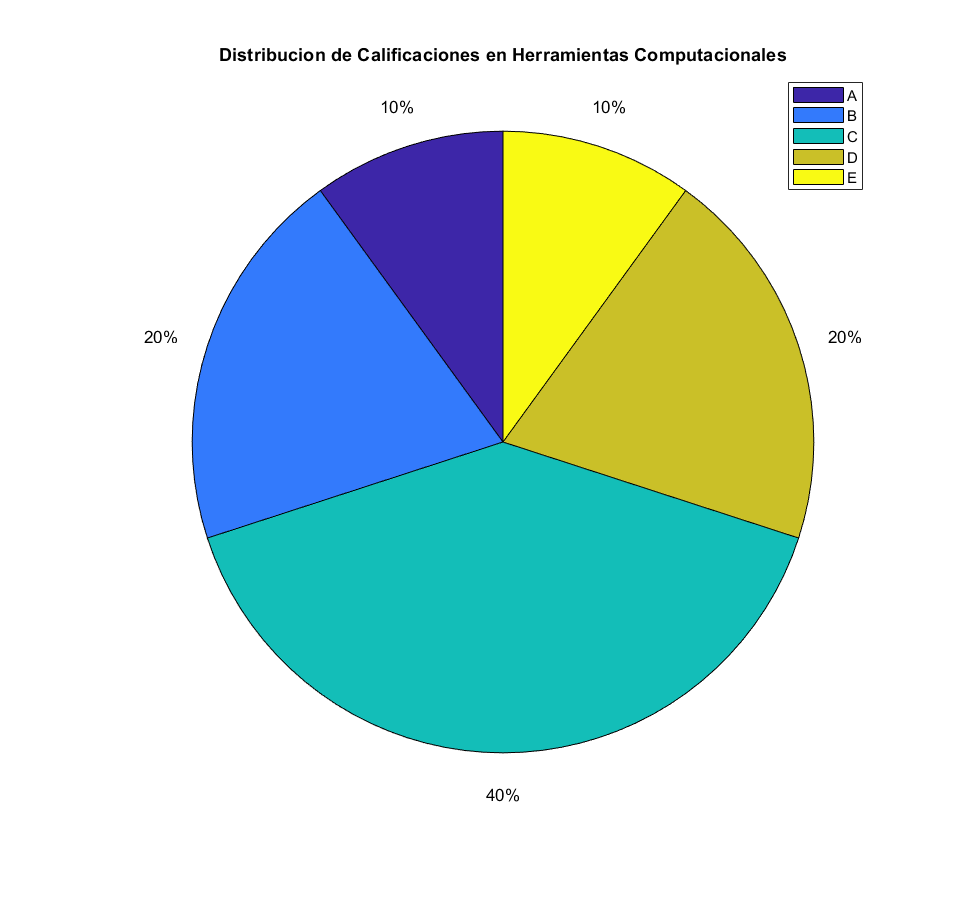
\includegraphics[width=\textwidth]{grafica20a.png}
	\end{figure*}
	
	\newpage
	
	\subsubsection{Grafica 2}
	
	\begin{figure*}[h]
		\centering
		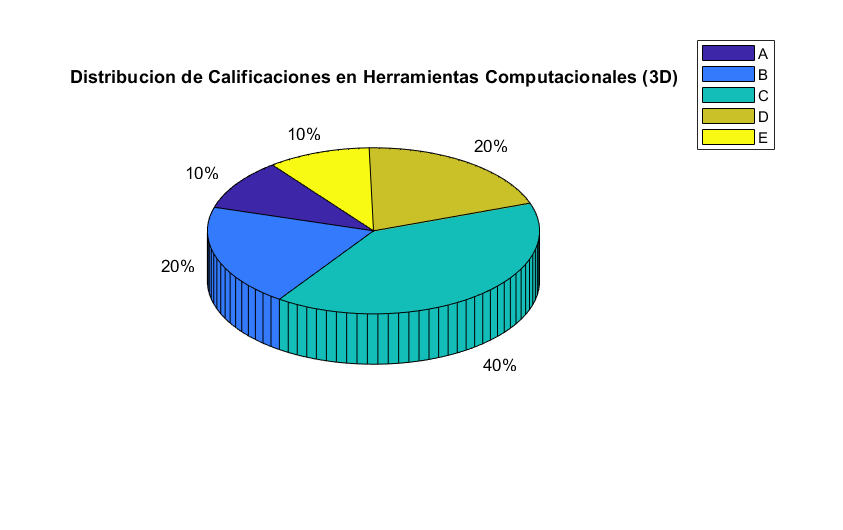
\includegraphics[width=\textwidth]{grafica20b.png}
	\end{figure*}
	
	\newpage
	
	\subsection{Problema 14}
	
	Cree un vector $x$ de valores desde $0$ hasta $20\pi$, con un espaciamiento de $\pi/100$. Defina los vectores $y$ y $z$ como
	
	$y = x \sin(x); z = x \cos(x)$
	
	\begin{enumerate}
		\item Cree una grafica $x - y$ de $x$ y $y$.
		\item Cree una grafica polar de $x$ y $y$.
		\item Cree una grafica lineal tridimensional de $x$, $y$ y $z$. No olvide un titulo y etiquetas.
	\end{enumerate}
	
	\subsubsection{Script21.m}
	
	\begin{lstlisting}

% Programa que genera 3 graficas; una cartesiana, una polar y una
% tridimencional.

x = 0:pi/100:20*pi;

y = x .* sin(x);
z = x .* cos(x);

figure;
plot(x, y, 'b-', 'LineWidth', 3);
xlabel('x');
ylabel('y');
title('Grafica x - y de x y y');

figure;
polarplot(x, y, 'c-', 'LineWidth', 3);
title('Grafica polar de x y y');

figure;
plot3(x, y, z, 'm-', 'LineWidth', 3);
xlabel('x');
ylabel('y');
zlabel('z');
title('Grafica tridimensional de x, y y z');

	\end{lstlisting}
	
	\subsubsection{Ejecución}
	
	\begin{lstlisting}
	>>Script21
	\end{lstlisting}
	
	\newpage
	
	\subsubsection{Grafica 1}
	
	\begin{figure*}[h]
		\centering
		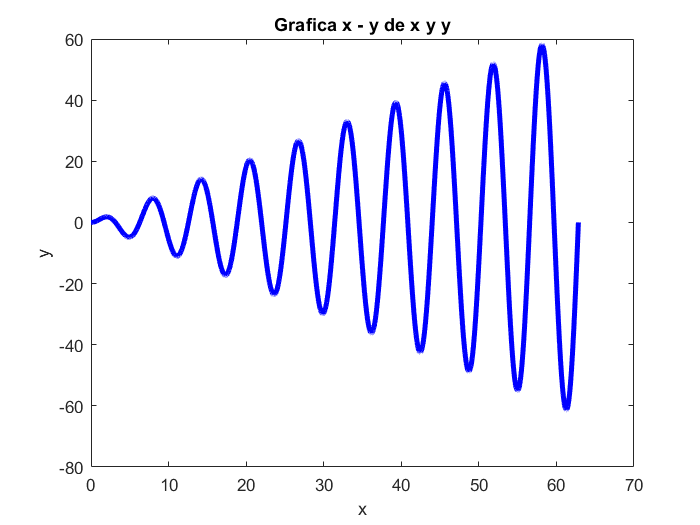
\includegraphics[width=\textwidth]{grafica21a.png}
	\end{figure*}
	
	\newpage
	
	\subsubsection{Grafica 2}
	
	\begin{figure*}[h]
		\centering
		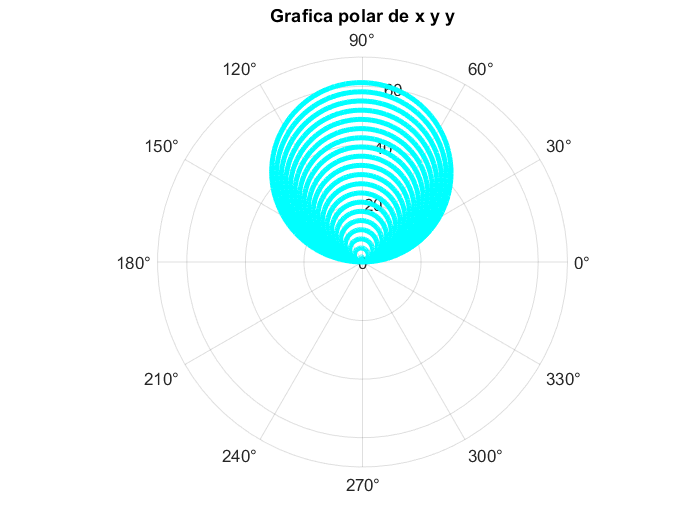
\includegraphics[width=\textwidth]{grafica21b.png}
	\end{figure*}
	
	\newpage
	
	\subsubsection{Grafica 3}
	
	\begin{figure*}[h]
		\centering
		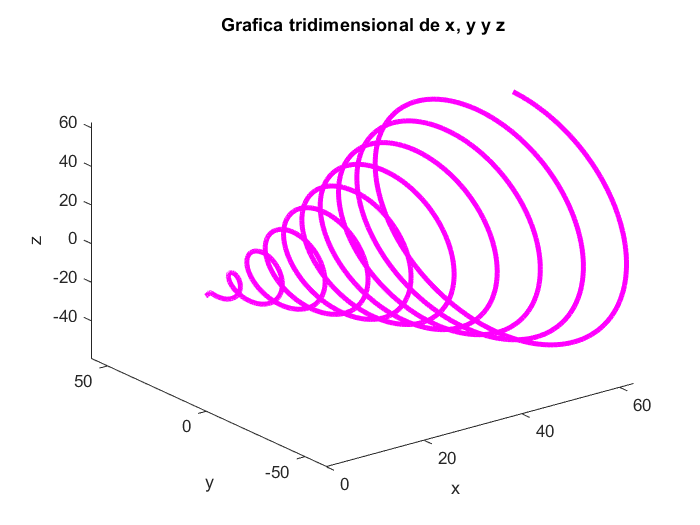
\includegraphics[width=\textwidth]{grafica21c.png}
	\end{figure*}
	
	\newpage
	
	\subsection{Problema 15}
	
	Cree vectores $x$ y $y$ desde $-5$ hasta $5$ con un espaciamiento de $0.5$. Use la función \textbf{meshgrid} para mapear $x$ y $y$ en dos nuevas matrices bidimensionales llamadas $X$ y $Y$ . Use sus nuevas matrices para calcular el vector $Z$, con magnitud
	
	\begin{equation*}
		Z = \sin(\sqrt{X^2 + Y^2})
	\end{equation*}
	
	\begin{itemize}
		\item Use la función de graficacion \textbf{mesh} para crear una grafica tridimensional de $Z$.
		\item Use la función de graficacion \textbf{surf} para crear una grafica tridimensional de $Z$.
		Compare los resultados que obtuvo con una sola entrada ($Z$) con los obtenidos con entradas para las tres dimensiones ($X$, $Y$, $Z$).
		\item Genere una grafica de contorno de $Z$.
		\item Genere una combinación de graficas de superficie y de contorno de $Z$.
	\end{itemize}
	
	\subsubsection{Script22.m}
	
	\begin{lstlisting}

% Programa que genera graficas en tres dimenciones.

x = -5:0.5:5;
y = -5:0.5:5;

[X, Y] = meshgrid(x, y);

Z = sin(sqrt(X.^2 + Y.^2));

figure;
mesh(Z);

figure;
surf(Z);

figure;
surf(X, Y, Z);

figure;
contour(Z);

figure;
surf(X, Y, Z);
hold on;
contour(X, Y, Z);
hold off;

	\end{lstlisting}
	
	\newpage
	
	\subsubsection{Grafica 1}
	
	\begin{figure*}[h]
		\centering
		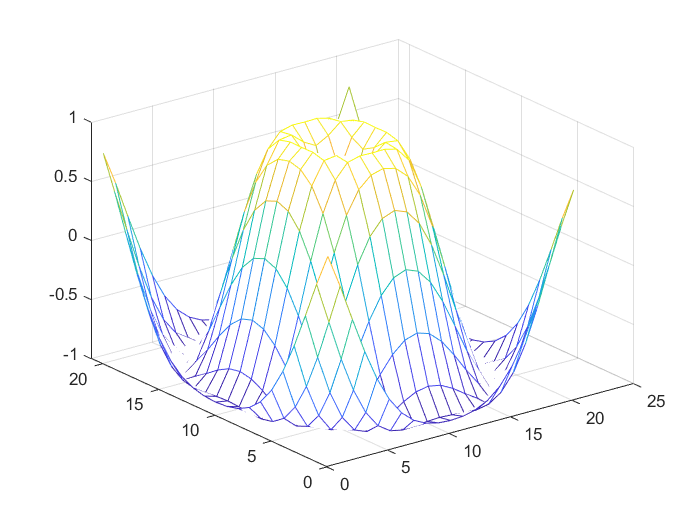
\includegraphics[width=\textwidth]{grafica22a.png}
	\end{figure*}
	
	\newpage
	
	\subsubsection{Grafica 2}
	
	\begin{figure*}[h]
		\centering
		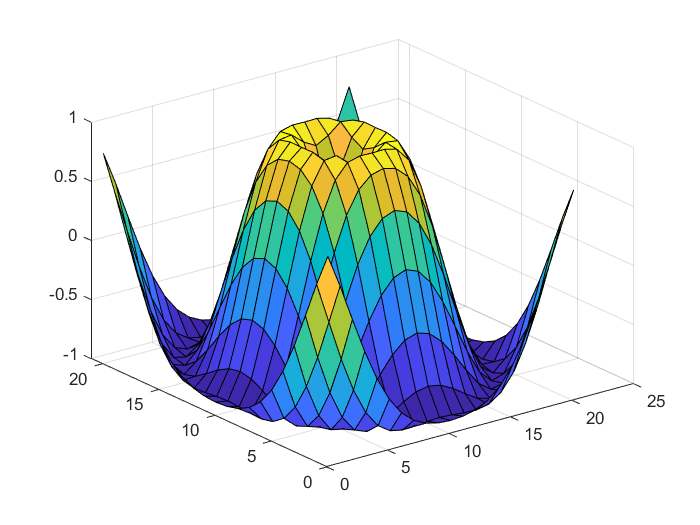
\includegraphics[width=\textwidth]{grafica22b.png}
	\end{figure*}
	
	\newpage
	
	\subsubsection{Grafica 3}
	
	\begin{figure*}[h]
		\centering
		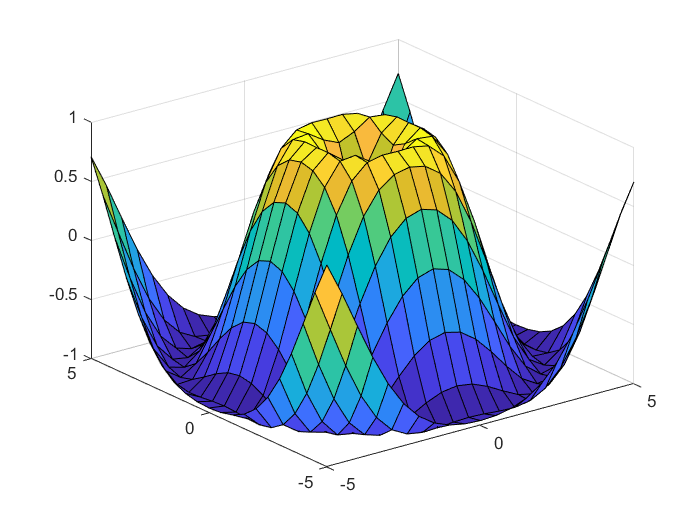
\includegraphics[width=\textwidth]{grafica22c.png}
	\end{figure*}
	
	\newpage
	
	\subsubsection{Grafica 4}
	
	\begin{figure*}[h]
		\centering
		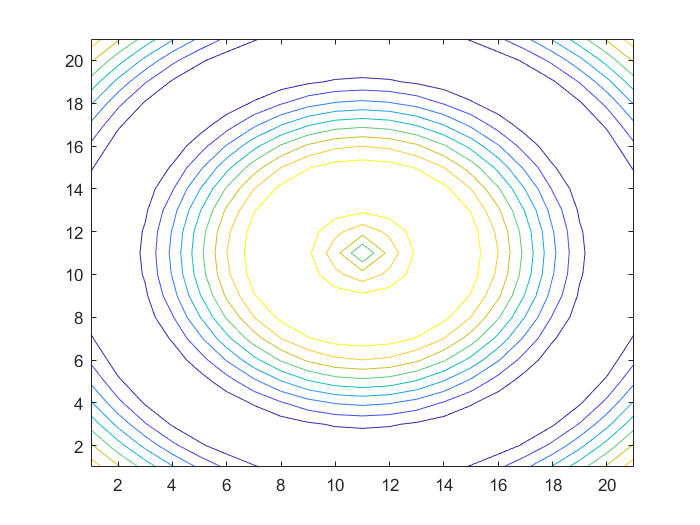
\includegraphics[width=\textwidth]{grafica22d.png}
	\end{figure*}
	
	\newpage
	
	\subsubsection{Grafica 5}
	
	\begin{figure*}[h]
		\centering
		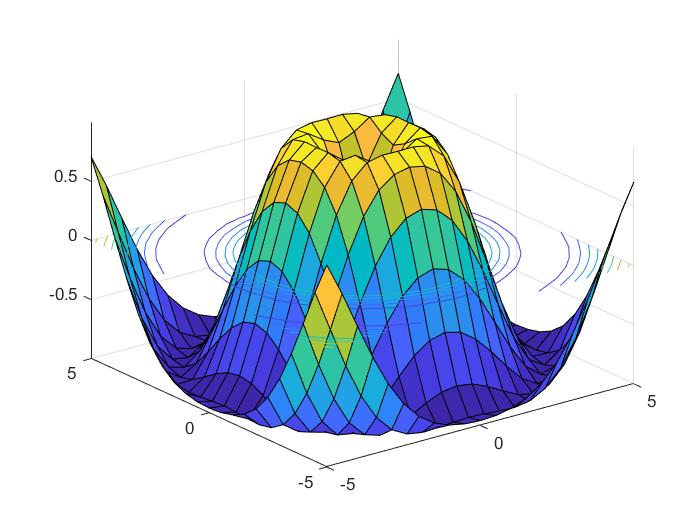
\includegraphics[width=\textwidth]{grafica22e.png}
	\end{figure*}
	
	\newpage
	
	\newpage
	\section{Conclusión}
	
	En conclusión, esta práctica es una oportunidad para aprender a utilizar las diferentes opciones que nos ofrece la interfaz de \textbf{MATLAB} para visualizar datos de forma clara y efectiva.
	
\end{document}